\title{\textbf{Geometry and Metric Structure of the\\ UNNS Arithmetic Graph}\\[6pt]
\large Sharp distance laws, scaling and power lifting, cycle structure, prime neighbourhoods and Fibonacci routes}
\author{UNNS Research Collective}
\date{Version 1.4 \,--\, 11 November 2026}

\begin{document}
\maketitle

\begin{abstract}
\noindent
Let $G$ be the undirected graph on the positive integers in which $kN$ is joined to $k(N+1)^2$ for all integers $k,N\ge1$.
This paper studies the metric geometry of $G$ as a mathematical object in its own right.
We prove that $G$ is simple and locally finite, that $\deg_G(x)=\tau(x)+\#\{q\ge2:q^2\mid x\}$ (so no vertex has degree $3$), and that $G$ is connected.
We prove three sharp distance laws: the largest distance between consecutive integers is $6$, between an integer and its double is $5$, and between consecutive squares is $5$.
The successor and consecutive-square upper bounds follow from explicit finite families of polynomial path identities (nine and $24$ respectively), whose intermediate states and cofactors are polynomials in a class parameter, certified to be positive integers for the whole class; the doubling upper bound follows by multiplicative scaling of a single five-edge path from $1$ to $2$. Sharpness is established by exact finite-ball certificates: each lower bound is the disjointness of two finite balls, computed by exact integer arithmetic.
We show that multiplication by $m$ is a non-expanding map of $G$, that a path from $x$ to $y$ lifts to a path from $x^k$ to $y^k$ at $k$ times the length, and that every prime has exactly the two neighbours $4p$ and $(p+1)^2$, so that distances between primes reduce to distances between four composite points.
$G$ is triangle-free with girth $4$ and odd girth $5$.
For consecutive Fibonacci numbers there is a uniform bound $\dist(F_k,F_{k+1})\le12$, obtained from twelve certified route families indexed by $k$ modulo $12$; these are route-length bounds, not shortest paths.
We also prove that $\dist(1,n)\le11\lfloor\log_2n\rfloor$, so the diameter of $\{1,\dots,n\}$ has an upper bound logarithmic in $n$, and we separate what the geometry of $G$ guarantees (reachability with uniformly bounded length) from what is extra information (selecting a route without a target).
All computations are reproduced here by new, independently written code; the earlier heavy verifications are inherited and are identified as not re-run.
\end{abstract}

\tableofcontents
\newpage

%=====================================================================
\section{Introduction}\label{sec:intro}
%=====================================================================
\subsection{The object}
The UNNS Substrate contains an arithmetic operation that nests a number $N$ into a number $M$ divisible by it,
\[
M\ \longmapsto\ M\,\frac{(N+1)^2}{N}\qquad(N\mid M).
\]
Read as a rule on the positive integers it is a partial function with many branches; its graph is the set of pairs
$\{kN,\ k(N+1)^2\}$, one for each cofactor $k\ge1$ and each $N\ge1$.
The \emph{UNNS arithmetic graph} $G$ is the undirected graph with these edges on the vertex set $\N_{>0}=\{1,2,3,\dots\}$.
Traversal is allowed in both directions: a forward step $+N$ multiplies by $(N+1)^2/N$, and an inverse step $-N$ multiplies by $N/(N+1)^2$. The value $N=1$ is permitted, so that $k\sim4k$ for every $k$.
This convention is deliberate and is used throughout; it differs from the forward-only, $N\ge2$ selector studied in the companion manuscript on autonomous aperiodicity, which asks a different question (what a rule with no target will generate) and is not used here.

The questions of this paper are those one asks of any infinite connected graph: what do neighbourhoods look like, how far apart can two vertices that are close \emph{as numbers} be, how do the arithmetic operations (scaling, powers) act on distance, and what are the shortest cycles.
We answer them completely where the arithmetic permits, with explicit proofs, and we state exactly where a statement rests on a finite computation.

\subsection{Results}
\begin{theorem}[Summary]\label{thm:summary}
\begin{enumerate}[label=(\alph*),itemsep=1pt]
\item \textbf{Structure.} $G$ is simple, locally finite and connected, with $\deg_G(x)=\tau(x)+\#\{q\ge2:q^2\mid x\}$; $\deg_G(1)=1$, every prime has degree $2$ with neighbours $4p$ and $(p+1)^2$, and no vertex has degree $3$. If $x\sim y$ and $x<y$ then $y/x\ge4$. (Theorems~\ref{thm:degree}, \ref{thm:connected}; degree formula and prime degree: \cite{u2tidyn}; connectivity follows from the successor bound of \cite{u1bnd}.)
\item \textbf{Successor distance.} $2\le \dist(n,n+1)\le6$ for every $n\ge1$, and $\dist(163,164)=6$. Hence $\sup_n\dist(n,n+1)=6$. (Theorem~\ref{thm:successor}; first established in \cite{u1bnd}.)
\item \textbf{Multiplicative geometry.} $\dist(ma,mb)\le\dist(a,b)$ and $\dist(x^k,y^k)\le k\,\dist(x,y)$. (Theorems~\ref{thm:scaling}, \ref{thm:lifting}; \cite{u2sq}.)
\item \textbf{Doubling.} $\dist(n,2n)\le5$ for all $n$, with equality at $n=1$; hence $\sup_n\dist(n,2n)=5$. (Theorem~\ref{thm:doubling}; first established in \cite{u2}.)
\item \textbf{Squares.} $\dist(n^2,(n+1)^2)\le5$ for all $n$, and $\dist(23^2,24^2)=5$; hence $\sup_n\dist(n^2,(n+1)^2)=5$. (Theorem~\ref{thm:squares}; first established in \cite{u2sq}.)
\item \textbf{Cycles.} $G$ is triangle-free, has girth $4$ (the cycle $2\!-\!8\!-\!36\!-\!9$) and odd girth $5$ (the cycle $6\!-\!24\!-\!96\!-\!784\!-\!27$). (Theorem~\ref{thm:girth}; triangle-freeness and odd girth $5$ in \cite{u3}, the corrected girth $4$ in \cite{u3cor}.)
\item \textbf{Primes.} For distinct primes, $\dist(p,q)=2+\min\dist(u,v)$ over $u\in\{4p,(p+1)^2\}$, $v\in\{4q,(q+1)^2\}$; $\dist(61,67)=7$ and $\dist(661,673)=8$, so $6$ is not a bound for primes. (Theorem~\ref{thm:primedist}; \cite{u2fp}.)
\item \textbf{Fibonacci routes.} $\dist(F_k,F_{k+1})\le12$ for all $k\ge2$, by twelve certified route families (one for each class of $k$ modulo $12$) and an exact table for $k\le29$. This is a bound on certified route length, not a statement that the routes are shortest. (Theorem~\ref{thm:fibonacci}; the twelve certified families are from \cite{u2fpsym}, which supplements \cite{u2fp}.)
\end{enumerate}
\end{theorem}
The three numbers $6,5,5$ in (b), (d), (e) are \emph{sharp}: each is the exact supremum, with a constructive upper bound valid for every $n$ and a computed lower bound at one explicit instance; the three laws were first established in \cite{u1bnd}, \cite{u2} and \cite{u2sq} respectively.

\subsection{Evidence levels}
Throughout, three kinds of statement are distinguished and labelled.
\begin{itemize}[itemsep=1pt]
\item \textbf{Proved.} A mathematical argument that a reader can check line by line; it may use the explicit finite tables of the appendices, whose entries are verified identities (see below).
\item \textbf{Certified.} A finite family of polynomial identities, checked with exact computer algebra, from which an infinite family of statements follows by an argument given in the text (Lemma~\ref{lem:certificate}). The reader can recheck each identity by hand or with any algebra system; no proof assistant was used.
\item \textbf{Computed.} A finite exact computation with integers (an exhaustive ball enumeration, a table of distances, a replay of routes). Lower bounds on distances are of this kind: they assert that two explicitly listed finite sets are disjoint.
\end{itemize}
Every statement carries one of these labels in its proof or in the status table of Section~\ref{sec:verification}.

\subsection{Relation to earlier releases}
The results of this paper were first established in earlier UNNS reports, collected at a fixed commit in~\cite{coll}: bounded successor distance (U1-BND~\cite{u1bnd}); doubling and the finite-control successor selector (U2-001~\cite{u2}); squares and power lifting (U2-SQ~\cite{u2sq}); the degree formula and prime-degree rigidity (U2-TI-DYN~\cite{u2tidyn}); primes and Fibonacci routes (U2-FP~\cite{u2fp} and its symbolic supplement U2-FP-SYM~\cite{u2fpsym}); and cycle structure (U3~\cite{u3}, which proves triangle-freeness and odd girth $5$, and the correction U3-COR~\cite{u3cor}, which establishes girth $4$).
Those releases are frozen and unchanged. The present manuscript is a single self-contained argument: the definitions, the proofs and the certificates needed to follow them are all given here, including the connectivity statement (which is a two-line consequence of the successor bound and is proved here), the degree formula, and a complete derivation of the three sharp bounds. All numerical and symbolic checks have been re-implemented from the definitions (Section~\ref{sec:verification}); where an earlier verification was heavy and is not repeated, this is stated and the archive hash is recorded. Section~\ref{ssec:provenance} states which release supports which statement.
We do not reproduce the topological study of finite history complexes of the same graph (GIG); that is a different subject. Here the graph is infinite and the object of study is its distance and cycle structure.

\subsection{Conventions}
$\N_{>0}$ denotes the positive integers; $\tau(x)$ is the number of divisors of $x$; $\dist$ is the graph distance in $G$ (the least number of edges of a path); $\Ball_r(v)$ is the closed ball of radius $r$ about $v$; a \emph{route} is a path given by a start vertex and signed labels $\pm N_1,\dots,\pm N_\ell$. Fibonacci numbers are $F_0=0,F_1=1,F_{j+1}=F_j+F_{j-1}$.

%=====================================================================
\section{The graph}\label{sec:graph}
%=====================================================================
\begin{definition}[The arithmetic graph]\label{def:G}
$V(G)=\N_{>0}$ and $E(G)=\bigl\{\{kN,\ k(N+1)^2\}:\ k,N\in\N_{>0}\bigr\}$.
\end{definition}
Since $kN<k(N+1)^2$ the two endpoints of every edge are distinct, so there are no loops.

\subsection{Moves}
For $x\in\N_{>0}$ and $N\in\N_{>0}$ define
\begin{align*}
&\text{forward move } +N:\quad x\mapsto x\,\frac{(N+1)^2}{N},\ \text{legal iff } N\mid x;\\
&\text{inverse move } -N:\quad x\mapsto x\,\frac{N}{(N+1)^2},\ \text{legal iff } (N+1)^2\mid x.
\end{align*}
\begin{lemma}[Moves are the edges]\label{lem:moves}
(i) $+N$ is legal at $x$ iff $x=kN$ for some $k\ge1$, and then its value is $k(N+1)^2$. (ii) $-N$ is legal at $y$ iff $y=k(N+1)^2$ for some $k\ge1$, and then its value is $kN$. (iii) The moves $+N$ and $-N$ are mutually inverse. Consequently $\{x,y\}\in E(G)$ iff $y$ is obtained from $x$ by one legal move.
\end{lemma}
\begin{proof} Immediate from the definition of $E(G)$ with cofactor $k=x/N$, respectively $k=y/(N+1)^2$. \end{proof}
We call $k$ the \emph{cofactor} of the move.

\begin{lemma}[Legality from integrality]\label{lem:legal}
Let $s,t,N$ be positive integers. If $tN=s(N+1)^2$ then $N\mid s$ and $+N$ carries $s$ to $t$. If $t(N+1)^2=sN$ then $(N+1)^2\mid s$ and $-N$ carries $s$ to $t$.
\end{lemma}
\begin{proof} $\gcd(N,(N+1)^2)=1$. From $tN=s(N+1)^2$ we get $N\mid s(N+1)^2$, hence $N\mid s$. From $t(N+1)^2=sN$ we get $(N+1)^2\mid sN$, hence $(N+1)^2\mid s$. \end{proof}
This lemma is what makes certification of identities simple: a step needs no separate legality check once source, target and label are positive integers satisfying the defining equation.

\subsection{Edge ratio and the label of an edge}
Put $\rho_N=(N+1)^2/N=N+2+1/N$.
\begin{lemma}[Edge ratio]\label{lem:ratio}
$\rho_1=4$ and $\rho_{N+1}-\rho_N=1-\frac1{N(N+1)}>0$; thus $N\mapsto\rho_N$ is strictly increasing and $\rho_N\ge4$ with equality only for $N=1$. If $x<y$ are adjacent then $y/x=\rho_N$ for a unique $N\ge1$ with $N\mid x$; this $N$ is the \emph{label} of the edge.
\end{lemma}
\begin{proof} The computation of $\rho_{N+1}-\rho_N$ is direct. If $x=kN$ and $y=k(N+1)^2$ then $y/x=\rho_N$; uniqueness of $N$ is the injectivity of $\rho$. \end{proof}
\begin{corollary}[Consecutive integers are never adjacent]\label{cor:nonadj}
If $x\sim y$ and $x<y$ then $y\ge4x$. In particular $n\not\sim n+1$ and $\dist(n,n+1)\ge2$ for all $n\ge1$.
\end{corollary}
\begin{proof} $(n+1)/n\le2<4\le\rho_N$ for every $n,N\ge1$. \end{proof}
The vertex $1$ is joined to $4$ only, and $2$ is not adjacent to $1$ or $3$.

\subsection{Neighbours and degrees}
\begin{theorem}[Neighbours and degree]\label{thm:degree}
For $x\ge1$ let $s(x)=\#\{q\ge2:q^2\mid x\}$. The neighbours of $x$ are
\[
\Nbr(x)=\Bigl\{\,x\frac{(N+1)^2}{N}:\ N\mid x\Bigr\}\ \cup\ \Bigl\{\,x\frac{q-1}{q^2}:\ q\ge2,\ q^2\mid x\Bigr\},
\]
the first set consisting of $\tau(x)$ distinct integers $>x$, the second of $s(x)$ distinct integers $<x$. Hence
\[
\deg_G(x)=\tau(x)+s(x).
\]
Consequently $G$ is locally finite; $\deg_G(1)=1$; $\deg_G(p)=2$ for every prime $p$; $\deg_G(x)\ge4$ for every composite $x$; and no vertex has degree $3$. A vertex has no neighbour below it iff $x$ is squarefree.
\end{theorem}
\noindent\emph{Source.} The neighbourhood description, the degree formula, the characterisation of primes as the vertices of degree $2$, and the absence of degree $3$ are established in U2-TI-DYN~\cite{u2tidyn}. The proof below is self-contained.
\begin{proof}
Forward moves from $x$ are $+N$ with $N\mid x$ (Lemma~\ref{lem:moves}); the value is $x\rho_N>x$ and, by Lemma~\ref{lem:ratio}, different $N$ give different values. Inverse moves are $-N$ with $(N+1)^2\mid x$; writing $q=N+1\ge2$ the value is $x(q-1)/q^2<x$, and distinct $q$ give distinct values because $q\mapsto(q-1)/q^2$ is strictly decreasing on $q\ge2$ (the two inverse moves $q<q'$ give $x\rho_{q-1}^{-1}$ and $x\rho_{q'-1}^{-1}$ with $\rho_{q-1}<\rho_{q'-1}$). Forward values exceed $x$ and inverse values are below $x$, so the two sets are disjoint and $\deg_G(x)=\tau(x)+s(x)$.
For $x=1$: $\tau=1$, $s=0$. For a prime $p$: $\tau=2$ and $s=0$ since $p$ is squarefree. If $x$ is composite then $\tau(x)\ge3$; $\tau(x)=3$ forces $x=p^2$, and then $s(x)\ge1$ (take $q=p$), so $\deg\ge4$; if $\tau(x)\ge4$ then $\deg\ge4$. Squarefree $x$ has no $q\ge2$ with $q^2\mid x$.
\end{proof}
\begin{example} $\Nbr(4)=\{1,16,18,25\}$: the forward moves $+1,+2,+4$ give $16,18,25$ and the inverse move $-1$ gives $1$; $\deg(4)=\tau(4)+s(4)=3+1=4$. $\Nbr(12)$ has $\tau(12)=6$ upward and $s(12)=1$ downward neighbour (from $q=2$), so $\deg(12)=7$.
\end{example}
The degree is unbounded (take $x$ with many divisors), but the neighbourhood of every vertex is explicitly computable from its factorisation; this is the engine behind every computation in this paper.
\begin{remark}[Prime rigidity]\label{rem:primerigid}
For a prime $p$ the only two legal moves are $+1$ (to $4p$) and $+p$ (to $(p+1)^2$). Every path through $p$ therefore enters and leaves $p$ by these two moves; we use this in Section~\ref{sec:cycles}.
\end{remark}
\noindent\emph{Source.} Prime neighbour rigidity is established in U2-FP~\cite{u2fp}; the degree-$2$ characterisation of primes is in U2-TI-DYN~\cite{u2tidyn}.

\subsection{Scale of the graph, and connectivity (forward reference)}
Edges multiply the value by at least $4$, but they can be traversed in both directions, so geodesics between nearby integers typically rise to a large intermediate value and return (Figure~\ref{fig:worked}). The graph is connected; the proof is two lines once the bound $\dist(n,n+1)\le6$ is available and is given as Theorem~\ref{thm:connected} in Section~\ref{sec:successor}. We stress that no argument for connectivity is needed beyond that bound, so the manuscript is self-contained on this point.

\begin{figure}[ht]\centering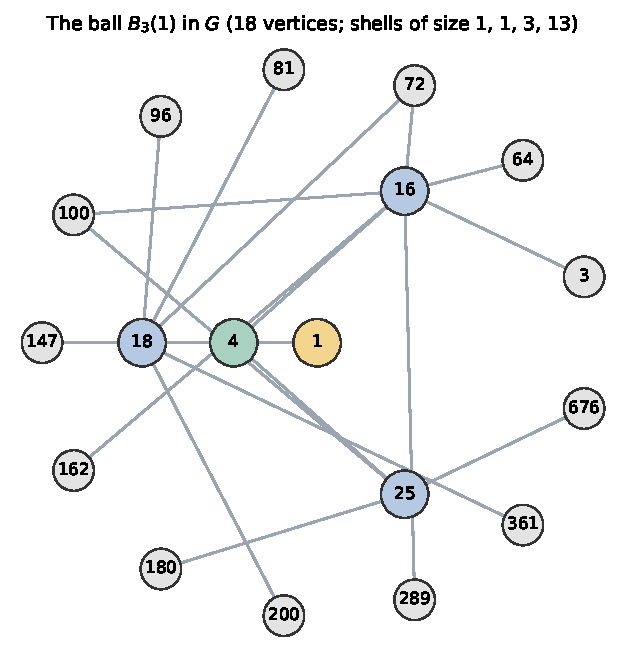
\includegraphics[width=.62\textwidth]{../figures/fig1_ball_of_one.pdf}
\caption{The ball $B_3(1)$: shells of size $1,1,3,13$ around the vertex $1$. The first step is forced ($1\to4$); the vertex $4$ has the three further neighbours $16,18,25$.}\label{fig:ball1}\end{figure}
\begin{figure}[ht]\centering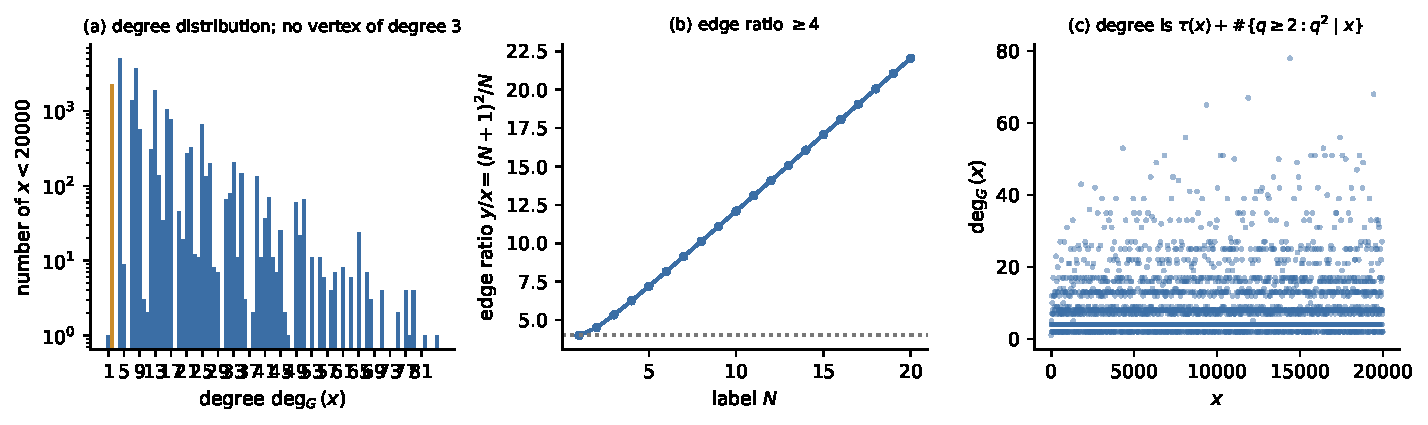
\includegraphics[width=\textwidth]{../figures/fig2_degrees_ratio.pdf}
\caption{(a) Degree distribution of the vertices $x<20000$; the degree-$2$ class is exactly the primes. (b) The edge ratio $\rho_N=(N+1)^2/N$. (c) The degree as a function of $x$; it equals $\tau(x)+s(x)$.}\label{fig:deg}\end{figure}

%=====================================================================
\section{Two tools: polynomial certificates and ball certificates}\label{sec:tools}
%=====================================================================
All sharp bounds in this paper use the same pair of devices: an \emph{upper bound} for all members of an infinite family by a single parametric path identity, and a \emph{lower bound} at one vertex pair by exhaustive enumeration of two small balls.

\subsection{Polynomial path certificates}
\begin{definition}[Parametric route]\label{def:param}
A \emph{parametric route} is a start state $s_0(t)\in\Z[t]$ together with signed labels $\sigma_iN_i(t)$, $N_i\in\Z[t]$, $\sigma_i\in\{+,-\}$, $i=1,\dots,\ell$, and polynomials $c_i(t)\in\Z[t]$ (cofactors) such that, writing $s_{i-1}$ for the state before step $i$,
\begin{align*}
\sigma_i=+:&\quad s_{i-1}=c_i\,N_i,\quad s_i=c_i\,(N_i+1)^2;\\
\sigma_i=-:&\quad s_{i-1}=c_i\,(N_i+1)^2,\quad s_i=c_i\,N_i
\end{align*}
as polynomial identities.
\end{definition}
\begin{lemma}[Certificate lemma]\label{lem:certificate}
Let $t_0\in\Z_{\ge0}$. Suppose that for every $i$ the polynomials $N_i(t)$ and $c_i(t)$ satisfy $N_i(t_0+u),\,c_i(t_0+u)\in\Z[u]$ with all coefficients non-negative and value $\ge1$ at $u=0$. Then for every integer $t\ge t_0$ the labelled sequence is a legal route in $G$ from $s_0(t)$ to $s_\ell(t)$ of length $\ell$.
\end{lemma}
\begin{proof} For an integer $t=t_0+u$ with $u\ge0$ every $N_i(t)$ and $c_i(t)$ is a positive integer: a polynomial with non-negative integer coefficients and constant term $\ge1$ is $\ge1$ on $u\ge0$. By Lemma~\ref{lem:moves}, step $i$ is the legal move $\sigma_iN_i(t)$ with cofactor $c_i(t)$, and it carries $s_{i-1}(t)$ to $s_i(t)$. \end{proof}
In practice one only has to exhibit, for each step, the cofactor $c_i(t)$; the identity $s_{i-1}=c_iN_i$ (or $c_i(N_i+1)^2$) is a division of polynomials. The \emph{certification} of a family consists of (i) these polynomial divisions with integer-coefficient quotients, (ii) the non-negativity test after the shift $t\mapsto t_0+u$, and (iii) the final identity $s_\ell(t)=$ target. All three are finite computations with polynomials of low degree and have been checked with exact symbolic algebra (Section~\ref{sec:verification}); the explicit tables of the appendices allow each to be checked by hand.

\subsection{Ball certificates}
\begin{lemma}[Meeting in the middle]\label{lem:mitm}
Let $a,b$ be vertices and $t\ge0$. If $\Ball_{\lceil t/2\rceil}(a)\cap\Ball_{\lfloor t/2\rfloor}(b)=\emptyset$ then $\dist(a,b)>t$.
\end{lemma}
\begin{proof} Suppose $\dist(a,b)=d\le t$ with geodesic $a=v_0,\dots,v_d=b$. Then $v_{\lceil d/2\rceil}$ lies within $\lceil d/2\rceil\le\lceil t/2\rceil$ of $a$ and within $d-\lceil d/2\rceil=\lfloor d/2\rfloor\le\lfloor t/2\rfloor$ of $b$. \end{proof}
Balls are enumerated by breadth-first search using Theorem~\ref{thm:degree}: $\Nbr(x)$ is computed from the prime factorisation of $x$. For a vertex pair at distance $\le6$ the balls have radii at most $3$; their sizes in the cases of this paper are collected in Table~\ref{tab:balls}.
\begin{table}[ht]\centering\small
\begin{tabular}{@{}lccccc@{}}\toprule
pair $(a,b)$ & claim & radii & $|\Ball(a)|$ & $|\Ball(b)|$ & balls disjoint\\\midrule
$(163,164)$ & $\dist\ge6$ & $3,\,2$ & $874$ & $123$ & yes\\
$(1,2)$ & $\dist\ge5$ & $2,\,2$ & $5$ & $9$ & yes\\
$(529,576)$ & $\dist\ge5$ & $2,\,2$ & $97$ & $562$ & yes\\
$(61,67)$ & $\dist\ge7$ & $3,\,3$ & $322$ & $721$ & yes\\
$(661,673)$ & $\dist\ge8$ & $4,\,3$ & $123993$ & $570$ & yes\\\bottomrule
\end{tabular}
\caption{Ball certificates for the sharp lower bounds. The radii refer to the two balls of Lemma~\ref{lem:mitm} with $t=\dist-1$. Each distance is attained: the matching path of that length is given in the text.}\label{tab:balls}\end{table}
\begin{remark}[Nature of the lower bounds]
A lower bound obtained this way is a statement that two explicitly given finite sets of integers are disjoint, established by exact integer arithmetic. It is not a formal proof in a proof assistant, and its correctness depends on the correct enumeration of $\Nbr(x)$ for every vertex $x$ in the ball. For this reason the computation has been run with two independent implementations, once in the earlier releases (Pollard-rho factorisation versus trial division) and once here (factorisation by computer algebra for the ball enumeration, with the neighbour function itself cross-checked against trial division and against the literal definition of $E(G)$ for all $x<1500$); all agree on every size and every distance quoted.
\end{remark}
